\subsection{Performance Evaluation}
\label{sec:evaluation}
We have compared the processing time of each user login in UPRESSO, with the original OIDC implementation (MITREid Connect) and SPRESSO which only hides the user's accessed RPs from IdP.

We run the evaluation on 3 physical machines connected in a separated 1Gbps network. A DELL OptiPlex 9020 PC (Intel Core i7-4770 CPU, 3.4GHz, 500GB SSD and 8GB RAM) with Window 10 prox64 works as the IdP. A ThinkCentre M9350z-D109 PC (Intel Core i7-4770s CPU, 3.1GHz, 128GB SSD and 8GB RAM) with  Window 10 prox64 servers as RP. The user adopts Chrome v75.0.3770.100 as the user agent on the Acer VN7-591G-51SS Laptop (Intel Core i5-4210H CPU, 2.9GHz, 128GB SSD and 8GB RAM) with  Windows 10 prox64. For SPRESSO, the extra trusted entity FWD is deployed on the same machine as IdP. 
%没有因为部署在同一个机器上使得开销变长,monitor指系统的监视器
The monitor demonstrates that the calculation and network processing of the IdP does not become a bottleneck (the load of CPU and network is in the moderate level).

We have measured the processing time for $1000$ login flows, and the the results is demonstrated in Figure~\ref{fig:evaluation}. The average time is 208 ms, 113 ms and 308 ms for UPRESSO, MITREid Connect and SPRESSO respectively. The result shows that UPRESSO proved the privacy protection without introducing prominent overhead.


For better comparison, we further divide a SSO login flow into 4 phases, which : 1. \textbf{Authentication request initiation} (Steps 1-2.5 in Figure~\ref{fig:process}), the period which starts before the user sends the login request and ends after the user receive the identity proof request transmitted from itself.
2. \textbf{Identity proof generation} (Step 4 in Figure~\ref{fig:process}), denoting the construction of identity proof at the IdP (excluding the user authentication); 3. \textbf{Identity proof transmition} (Steps 5.1-5.3 in Figure~\ref{fig:process}), for transmitting the proof from the IdP to the RP with the user's help; and 4. \textbf{Identity proof verification} (Steps 6 in Figure~\ref{fig:process}), for the RP  verifying and parsing the proof for the user's $Account$. 

\begin{figure}
  \centering
  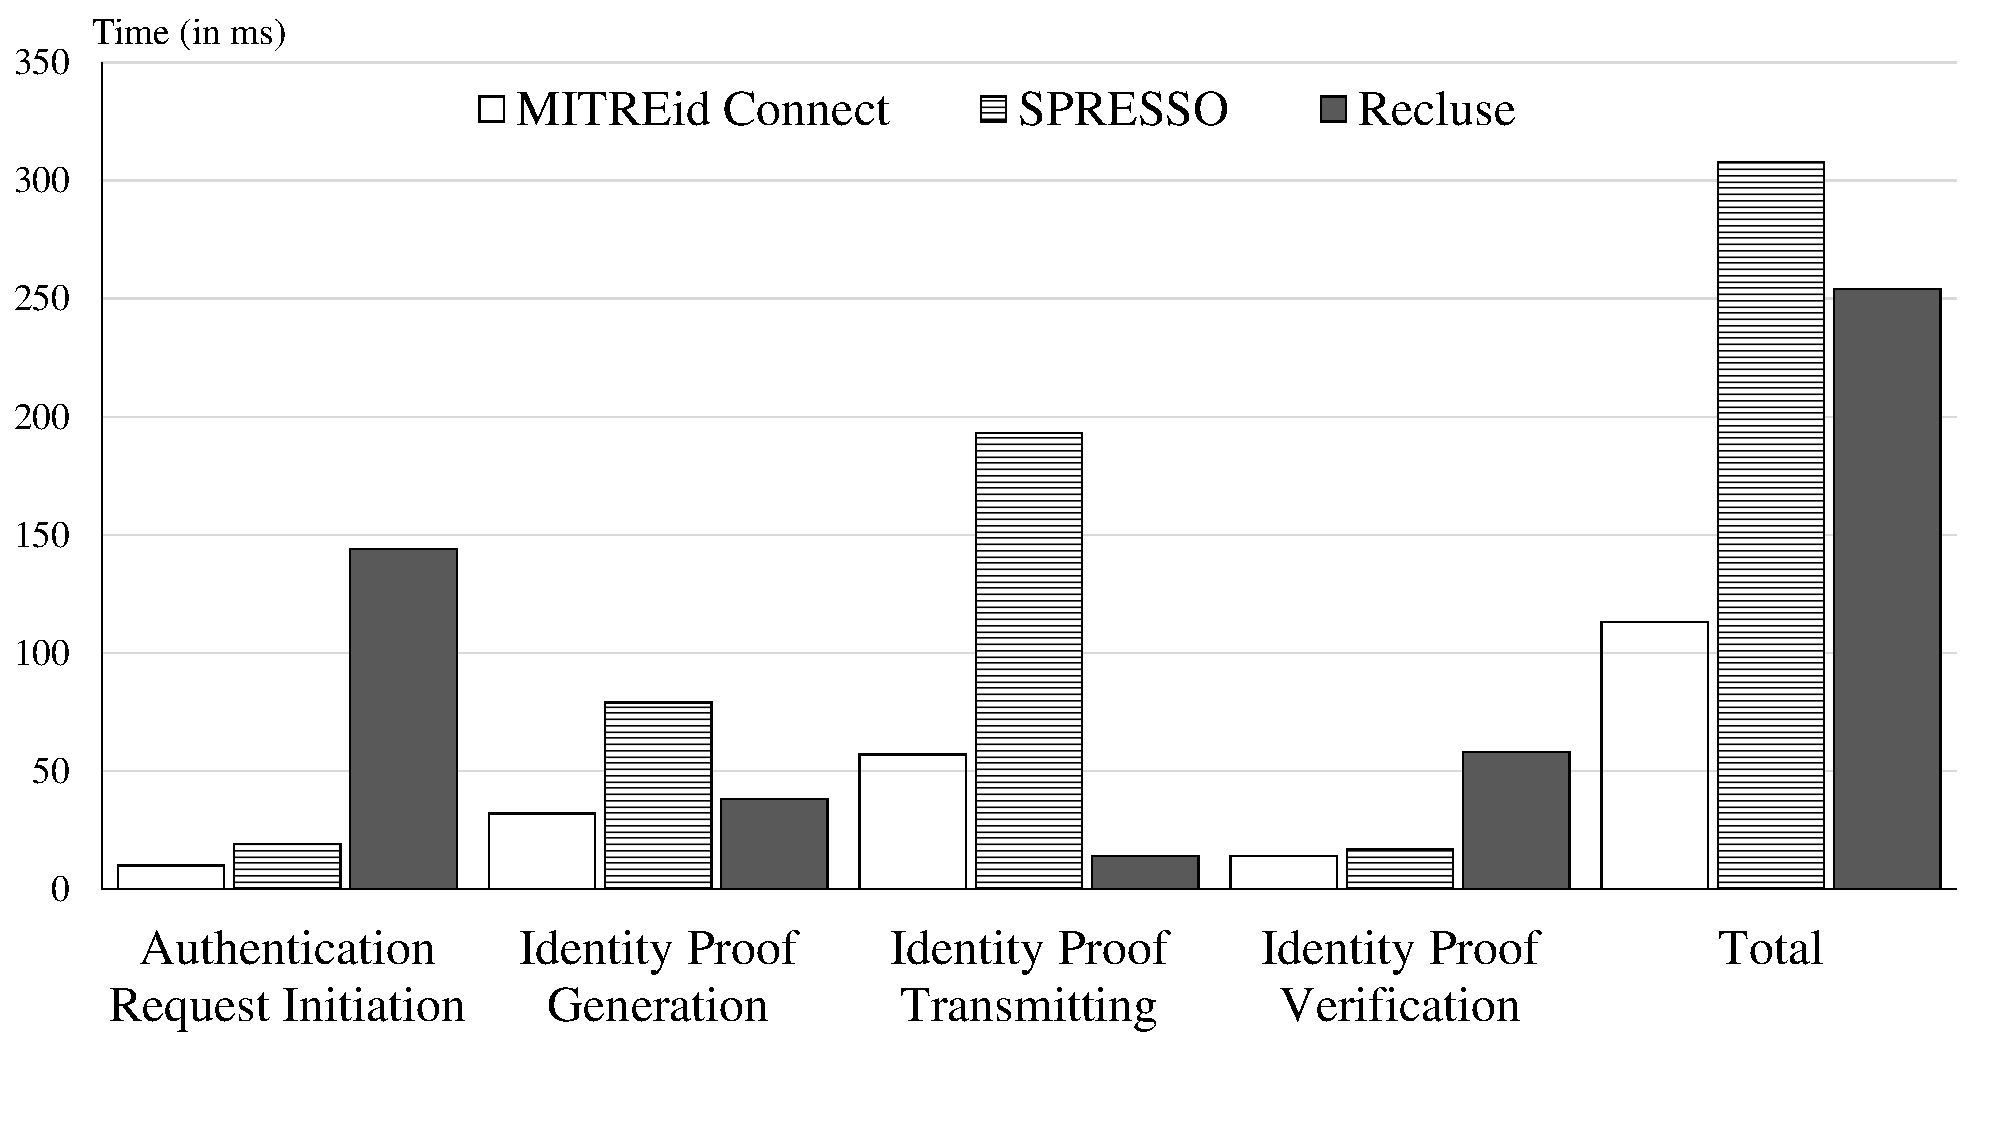
\includegraphics[width=\linewidth]{fig/evaluation2.pdf}
  \caption{The Evaluation.}
  \label{fig:evaluation}
\end{figure}
In the authentication request initiation, as UPRESSO need negotiate the $PID_{RP}$ (containing 1 modular exponentiation at the user and 2 at the RP) and renew the RP identifier at IdP, it should require the longest time cost. And SPRESSO has to obtain the public information from IdP and encrypt its domain (as the RP identifier), it should result the slight overhead compared with MITREid Connect. Finally, the evaluation shows that MITREid Connect requires the shortest time (10 ms), UPRESSO needs 98 ms and SPRESSO needs 19 ms.

For identity proof generation, UPRESSO need the extra time cost for the generation of $PID_U$ compared with MITREid Connect and SPRESSO. However, the evaluation shows that SPRESSO requires the longest time in this stage, and finally the time cost is found caused by the signature generation as SPRESSO is implemented with JavaScript while the others are using Java. In this stage, MITREid Connect needs 32 ms, UPRESSO needs an extra 6 ms and SPRESSO requires 71 ms. 

For identity proof transmission, UPRESSO should need the shortest time among these competitors, as it only need the chrome extension to relay the identity proof from the IdP to RP. MITREid Connect provides the proof as a fragment component (i.e., proof is preceded by \#) to RP to avoid the reload of RP document, and RP uses the JavaScript code to send the proof to the background server, which result that the time cost should be at a moderate level. The transmitting in SPRESSO is much complicated: The user's browser creates an iframe of the trusted entity (FWD), downloads the JavaScript from FWD, who obtains the RP's correct URL through a systematic decryption and communicates with the parent opener (also RP's document, but avoiding leaking RP to IdP) and RP's document through 3 post messages. The evaluation result shows that MITREid Connect needs 57 ms, UPRESSO needs only 14 ms and SPRESSO needs about 193 ms.

In identity proof verification, UPRESSO needs the extra time for calculation of $Account$ and signature verification compared with MITREid and SPRESSO. Therefore, the evaluation result is that MITREid Connect needs 14 ms, UPRESSO needs 58 ms and SPRESSO requires 17 ms.



